\documentclass[aspectratio=169, 12pt]{beamer}

% --- NOTES SETUP ---
% Comment out for final submission (no speaker notes)
% \usepackage{pgfpages}
% \setbeameroption{show notes on second screen=right} % Shows notes on the right side

% Theme - Modern but compatible
\usetheme{Boadilla}
\usecolortheme{whale}
% Add some modern touches
\setbeamertemplate{navigation symbols}{}  % Remove navigation symbols
% Custom footline that respects [noframenumbering]
\setbeamertemplate{footline}{
  \leavevmode%
  \hbox{%
  \begin{beamercolorbox}[wd=\paperwidth,ht=2.25ex,dp=1ex,right]{date in head/foot}%
    \usebeamerfont{date in head/foot}\insertframenumber{} / \inserttotalframenumber\hspace*{2ex}
  \end{beamercolorbox}}%
  \vskip0pt%
}

% Packages
\usepackage{graphicx}
\usepackage{tikz}
\usepackage{booktabs}
\usepackage{amsmath}
\usepackage{fontawesome5}
\usepackage{colortbl}
\usepackage{tcolorbox}

% Load TikZ libraries
\usetikzlibrary{shadows, calc, shapes, positioning}

% Path to your images
\graphicspath{{./images/}}

% Meta
\title[Cognitive MRI of AI Conversations]{Cognitive MRI of AI Conversations:\\A Single-User Case Study}
\subtitle{Revealing the Hidden Topology of Thought}
\author{Alex Towell \and John Matta}
\institute[SIUE]{Southern Illinois University Edwardsville}
\date{}

\begin{document}

%---------------------------------------------------------
% 1. Title
%---------------------------------------------------------
\begin{frame}
    \setlength{\columnsep}{18pt} % horizontal gap between the two blocks
    \begin{columns}[T]
        \column{0.65\textwidth}
        \vspace{0.5cm}

        {\LARGE\textbf{Cognitive MRI of AI Conversations:}}\\[0.3cm]
        {\LARGE\textbf{A Single-User Case Study}}\\[0.5cm]

        {\large A single-user ``cognitive MRI'' and how to scale it up}\\[0.8cm]

        {\large Alex Towell \quad John Matta}\\[0.3cm]
        {\normalsize Southern Illinois University Edwardsville}\\[0.2cm]
        {\normalsize \texttt{\{atowell,jmatta\}@siue.edu}}\\[0.8cm]

        {\footnotesize Code \& Data: \url{github.com/queelius/chatgpt-complex-net}}

        \column{0.35\textwidth}
        \vspace{1cm}
        \centering
        % Image filename
        \includegraphics[width=0.9\textwidth]{logo_cna2025_textblue.png}
    \end{columns}

    \note{
        \textbf{Slide 1: Title (30s)}
        \begin{itemize}
            \item \textbf{Hook:} ``Good morning. We often think of our interactions with AI as just `chats'---fleeting lines of text. But what if we treated them as a dataset of \textit{thought}?''
            \item \textbf{Core Question:} ``Can we take the linear logs of a single user and reconstruct the `shape' of their knowledge?''
            \item \textbf{Analogy:} ``We call this a \textbf{Cognitive MRI}. Just as an MRI images the physical structure of the brain from magnetic signals, we are imaging the \textit{conceptual} structure of the mind from semantic signals.''
            \item \textbf{Bridge (5s):} ``But before we dive into one user's map, let's understand why this matters at a planetary scale.''
        \end{itemize}
    }
\end{frame}

%---------------------------------------------------------
% 2. NEW: Why Now? The Scale of the Opportunity
%---------------------------------------------------------
\begin{frame}{Why Now? The Scale of the Opportunity}
    \begin{columns}[T]
        % LEFT: Visual representation of scale
        \column{0.5\textwidth}
        \centering
        \vspace{0.3cm}

        \textbf{1.7 Billion ChatGPT Users}

        \vspace{0.3cm}

        % TikZ: Globe with user icons
        \begin{tikzpicture}[scale=1.2]
            % Globe
            \draw[thick, blue!40] (0,0) circle (1.5cm);
            \draw[thick, blue!40] (0,0) ellipse (1.5cm and 0.5cm);
            \draw[thick, blue!40] (-1.5,0) arc (180:360:1.5cm and 1.5cm);

            % User icons scattered
            \foreach \angle/\radius in {30/1.2, 80/1.3, 130/1.1, 200/1.3, 260/1.2, 310/1.4} {
                \node[blue!60, font=\small] at (\angle:\radius) {\faUser};
            }

            % Central emphasis
            \node[font=\large, text=blue!80!black, align=center] at (0,-2.3) {
                \textbf{Global Scale}\\
                \scriptsize Unprecedented access to\\
                \scriptsize cognitive processes
            };
        \end{tikzpicture}

        \column{0.5\textwidth}
        \vspace{0.2cm}

        \textbf{Why This Matters}

        \vspace{0.2cm}

        % Comparison table
        \small
        \begin{tabular}{@{}lcc@{}}
            \toprule
            \textbf{Dataset Type} & \textbf{Scale} & \textbf{Process?} \\
            \midrule
            Citation Networks & $10^8$ papers & \textcolor{red}{No} \\
            Social Networks & $10^9$ users & \textcolor{red}{No} \\
            \rowcolor{green!10}
            LLM Conversations & $10^9$ users & \textcolor{green!60!black}{\textbf{Yes}} \\
            \bottomrule
        \end{tabular}

        \vspace{0.5cm}

        \begin{block}{\small First-Time Opportunity}
            \scriptsize
            Traditional datasets capture \textbf{outputs} (papers, posts).\\[0.2em]
            LLM logs capture the \textbf{iterative reasoning process} at global scale.
        \end{block}
    \end{columns}

    \note{
        \textbf{Slide 2: Scale \& Stakes (45s)}
        \begin{itemize}
            \item \textbf{Context:} ``Before we dive into methods, why does this matter?''
            \item \textbf{Scale:} ``ChatGPT has 1.7 billion users. Each one generating conversational traces of their thought process.''
            \item \textbf{Uniqueness:} ``Traditional datasets---citations, social networks---only capture the \textit{output}. They don't capture the iterative reasoning.''
            \item \textbf{Opportunity:} ``This is the first time in history we have access to the \textit{process} at global scale.''
            \item \textbf{Bridge to Methods:} ``Today we'll show a single-user case study. But the method generalizes. Imagine mapping the collective knowledge structure of entire research communities.''
        \end{itemize}
    }
\end{frame}

%---------------------------------------------------------
% 3. The Big Picture - EXTERNALIZED COGNITION
%---------------------------------------------------------
\begin{frame}{The Big Picture: Externalized Cognition}
    \begin{columns}[T]
        % --- LEFT COLUMN: The Narrative ---
        \column{0.55\textwidth}
        \small
        \textbf{AI conversations are not just chat logs.}

        \vspace{0.1cm}
        We view them through the lens of \textbf{Distributed Cognition}:
        \begin{itemize}
            \setlength\itemsep{0.1em}
            \item \textbf{Thinking Out Loud:} The user offloads cognitive load to the machine.
            \item \textbf{The Iterative Loop:} Ideas aren't just ``retrieved''; they are constructed through dialogue.
        \end{itemize}

        % CRITICAL FIX: Negative spacing to pull the block up
        \vspace{-0.3cm}

        \begin{alertblock}{The ``Cognitive Dark Matter''}
            \footnotesize
            Standard archives preserve the \emph{result} (the paper). \\
            LLM logs capture the \emph{process}---the false starts, synthesis, reasoning.
        \end{alertblock}

        % --- RIGHT COLUMN: The "Iceberg" Graphic ---
        \column{0.45\textwidth}
        \centering
        \begin{tikzpicture}[scale=0.95, transform shape]
            % --- WATERLINE ---
            \draw[dashed, gray, thick] (-2.5, 0) -- (2.5, 0);
            \node[fill=white, text=gray, font=\scriptsize] at (0,0) {Visibility Threshold};

            % --- TOP: THE ARTIFACT (The Paper) ---
            \node[anchor=south] at (0, 0.5) {
                \begin{tikzpicture}
                    % Paper Icon with Shadow
                    \draw[fill=white, drop shadow] (0,0) rectangle (1.2, 1.6);
                    % Text lines
                    \foreach \y in {1.2, 1.0, ..., 0.4} {
                        \draw[gray!50, thick] (0.2, \y) -- (1.0, \y);
                    }
                    \node[font=\tiny, align=center] at (0.6, -0.4) {\textbf{The Product}\\(Linear, Polished)};
                \end{tikzpicture}
            };

            % --- BOTTOM: THE PROCESS (The Network) ---
            \begin{scope}[yshift=-0.5cm]
                % Center Coordinate
                \coordinate (origin) at (0,-1.5);

                % Explicitly define nodes
                \path (origin) -- +(0:0.8) node[circle, fill=blue!20, inner sep=1.5pt] (n1) {};
                \path (origin) -- +(45:1.2) node[circle, fill=blue!20, inner sep=1.5pt] (n2) {};
                \path (origin) -- +(90:0.6) node[circle, fill=blue!20, inner sep=1.5pt] (n3) {};
                \path (origin) -- +(135:1.0) node[circle, fill=blue!20, inner sep=1.5pt] (n4) {};
                \path (origin) -- +(180:0.9) node[circle, fill=blue!20, inner sep=1.5pt] (n5) {};
                \path (origin) -- +(225:1.3) node[circle, fill=blue!20, inner sep=1.5pt] (n6) {};
                \path (origin) -- +(270:0.7) node[circle, fill=blue!20, inner sep=1.5pt] (n7) {};
                \path (origin) -- +(315:1.1) node[circle, fill=blue!20, inner sep=1.5pt] (n8) {};
                \path (origin) -- +(10:1.8) node[circle, fill=blue!20, inner sep=1.5pt] (n9) {};
                \path (origin) -- +(190:1.6) node[circle, fill=blue!20, inner sep=1.5pt] (n10) {};

                % Central Hubs
                \node[circle, fill=blue!40, inner sep=2.5pt] (hub1) at (0.2,-1.2) {};
                \node[circle, fill=blue!40, inner sep=2.5pt] (hub2) at (-0.3,-1.8) {};

                % Connections
                \draw[gray!60] (hub1) -- (n1); \draw[gray!60] (hub1) -- (n2);
                \draw[gray!60] (hub1) -- (n3); \draw[gray!60] (hub1) -- (hub2);
                \draw[gray!60] (hub2) -- (n4); \draw[gray!60] (hub2) -- (n5);
                \draw[gray!60] (hub2) -- (n6); \draw[gray!60] (n7) -- (n8);
                \draw[gray!60] (n1) -- (n8);   \draw[gray!60] (n4) -- (n9);
                \draw[gray!60] (n5) -- (n10);  \draw[gray!60] (hub1) -- (n7);

                \node[font=\tiny, align=center, text=blue!60!black] at (0, -3.5) {\textbf{The Process}\\(Networked, Exploratory)};
            \end{scope}

            % Connecting Arrow
            \draw[<-, thick, gray, dashed] (0.8, 0.2) to[bend left=45] (1.5, -1.5);
            \node[font=\tiny, text=gray, rotate=-90] at (2.2, -0.8) {Generated From};

        \end{tikzpicture}
    \end{columns}

    \note{
        \textbf{Slide 3: The Iceberg (1 min)}
        \begin{itemize}
            \item \textbf{Opening (15s):} ``We view this through the lens of \textbf{Distributed Cognition}---Hutchins' idea that thinking doesn't happen just in your head. It happens \textit{between} you and your tools.''
            \item \textbf{Point to Graphic - Above Waterline (20s):} [GESTURE TO TOP] ``What usually gets archived? The polished output. The paper. Linear, clean, final. This is what lives above the visibility threshold.''
            \item \textbf{Point to Graphic - Below Waterline (20s):} [GESTURE TO NETWORK BELOW] ``But below the surface? The actual thinking process. It's messy. It's networked. False starts, synthesis steps, backtracking. This is what we call the `Cognitive Dark Matter.' Usually invisible.''
            \item \textbf{The Opportunity (15s):} ``LLM logs capture this process for the first time. The iterative dialogue, the reasoning loop. Not just the destination---the journey.''
            \item \textbf{Bridge (5s):} ``So how do we make the invisible visible? Let me show you the transformation.''
        \end{itemize}
    }
\end{frame}

%---------------------------------------------------------
% 4. From Log to "Cognitive MRI"
%---------------------------------------------------------
\begin{frame}{From Log to a ``Cognitive MRI''}
    \centering
    \textbf{Transforming Linear Time into Semantic Topology}

    \vspace{0.1cm} % Reduced vertical spacing

    \begin{columns}[T]
        % --- LEFT: THE LINEAR LOG ---
        \column{0.45\textwidth}
        \centering
        \textbf{\textcolor{gray}{1. The Linear Log}} \\
        \scriptsize \textit{(Chronological Sequence)}

        \vspace{0.1cm}

        % Reduced scale to 0.7 to save vertical space
        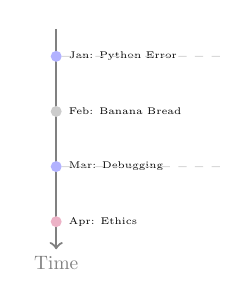
\begin{tikzpicture}[scale=0.7, transform shape]
            % Timeline arrow
            \draw[->, thick, gray] (0, 4) -- (0, 0) node[below] {Time};

            % Time Nodes
            \node[circle, fill=blue!30, inner sep=2pt, label=right:\tiny{Jan: Python Error}] (t1) at (0, 3.5) {};
            \node[circle, fill=gray!40, inner sep=2pt, label=right:\tiny{Feb: Banana Bread}] (t2) at (0, 2.5) {};
            \node[circle, fill=blue!30, inner sep=2pt, label=right:\tiny{Mar: Debugging}] (t3) at (0, 1.5) {};
            \node[circle, fill=purple!30, inner sep=2pt, label=right:\tiny{Apr: Ethics}] (t4) at (0, 0.5) {};

            % Dotted connections
            \draw[gray!30, dashed] (t1) -- (3, 3.5);
            \draw[gray!30, dashed] (t3) -- (3, 1.5);
        \end{tikzpicture}

        % --- MIDDLE: THE TRANSFORMATION ---
        \column{0.1\textwidth}
        \centering
        \vspace{1.2cm} % Adjusted for new scale
        
\begin{tikzpicture}[scale=0.7, transform shape]
            \draw[->, ultra thick, blue!50] (0,0) -- (0.8,0);
        \end{tikzpicture}\\
        \tiny \textbf{Embed}\\ \textbf{\& Link}

        % --- RIGHT: THE SEMANTIC NETWORK ---
        \column{0.45\textwidth}
        \centering
        \textbf{\textcolor{blue}{2. The Cognitive MRI}} \\
        \scriptsize \textit{(Semantic Topology)}

        \vspace{0.1cm}

        % Reduced scale to 0.7
        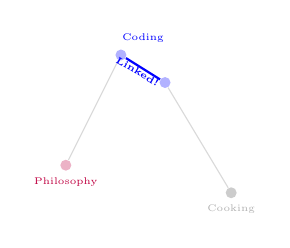
\begin{tikzpicture}[scale=0.7, transform shape]
            % Network Nodes
            \node[circle, fill=blue!30, inner sep=2pt] (n1) at (0, 3) {}; % Python
            \node[circle, fill=blue!30, inner sep=2pt] (n3) at (0.8, 2.5) {}; % Debugging
            \node[font=\tiny, text=blue] at (0.4, 3.3) {Coding};

            \node[circle, fill=gray!40, inner sep=2pt] (n2) at (2, 0.5) {}; % Banana Bread
            \node[font=\tiny, text=gray!60] at (2, 0.2) {Cooking};

            \node[circle, fill=purple!30, inner sep=2pt] (n4) at (-1, 1) {}; % Ethics
            \node[font=\tiny, text=purple] at (-1, 0.7) {Philosophy};

            % Edges
            \draw[thick, blue] (n1) -- (n3); % The link hidden in time!
            \draw[gray!30] (n1) -- (n4);
            \draw[gray!30] (n3) -- (n2);

            % Highlight the link
            \node[font=\tiny, text=blue, rotate=-30] at (0.3, 2.7) {\textbf{Linked!}};
        \end{tikzpicture}
    \end{columns}

    % Negative spacing to pull the block up away from the footer
    \vspace{-0.2cm}

    \begin{block}{The Insight}
        \footnotesize % Smaller font to ensure it fits
        Distance in \textbf{Time} $\neq$ Distance in \textbf{Thought}.\\
        The network reconnects ideas (e.g., two coding sessions months apart) that the linear log separates.
    \end{block}

    \note{
        \textbf{Slide 4: From Log to MRI (45s)}
        \begin{itemize}
            \item \textbf{Point to Left Side (15s):} [GESTURE TO TIMELINE] ``Here's the raw log. Chronological. January: Python error. February: Banana bread recipe. March: More Python debugging. April: Ethics discussion. Time flows downward.''
            \item \textbf{Point to Transformation Arrow (10s):} [GESTURE TO ARROW] ``Now we embed each conversation semantically and link by similarity, not by time.''
            \item \textbf{Point to Right Side - The Clustering (15s):} [GESTURE TO NETWORK] ``What happens? The two Python sessions---January and March---snap together in the network. They were months apart in time, but they're neighbors in semantic space. Banana bread stays isolated. Ethics forms its own cluster.''
            \item \textbf{The Key Insight (5s):} ``Distance in time does not equal distance in thought. The network reveals the true topology of your knowledge.''
        \end{itemize}
    }
\end{frame}

%---------------------------------------------------------
% 5. Pipeline: Intuition over Math
%---------------------------------------------------------
\begin{frame}{Method: Capturing Intent}
    \textbf{The Challenge:} AI responses are verbose and generic.\\
    \textbf{The Solution:} Focus on the human.

    \vspace{0.2cm}

    \begin{columns}[T]
        \column{0.5\textwidth}
        \begin{block}{The ``Signal'' is the User}
            \begin{itemize}
                \item We separate \textbf{User Prompts} from \textbf{AI Replies}.
                \item \textbf{Weighting:} We prioritize the user's voice (2:1 ratio).
                \item \textbf{Result:} The network connects conversations based on \emph{your} intent, not the AI's boilerplate.
            \end{itemize}
        \end{block}

        \vspace{0.2cm}
        {\tiny *Embeddings generated via nomic-embed-text (8k context).}

        \column{0.5\textwidth}
        \centering
        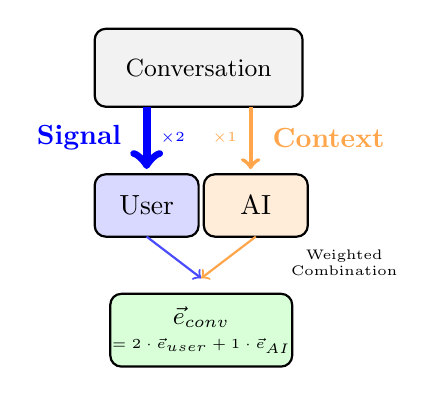
\begin{tikzpicture}[scale=0.66]
            % Conversation box
            \draw[rounded corners, thick, fill=gray!10] (0,5.5) rectangle (4,7);
            \node[align=center] at (2,6.25) {\small Conversation};

            % Separate arrows with VISUAL WEIGHTING
            % User arrow (THICKER - double weight)
            \draw[->, line width=3pt, blue] (1,5.5) -- (1,4.3);
            \node[blue, font=\bfseries] at (-0.3,4.9) {Signal};
            \node[blue, font=\tiny] at (1.5,4.9) {$\times 2$};

            % AI arrow (THINNER - single weight)
            \draw[->, line width=1.5pt, orange!70] (3,5.5) -- (3,4.3);
            \node[orange!70, font=\bfseries] at (4.5,4.9) {Context};
            \node[orange!70, font=\tiny] at (2.5,4.9) {$\times 1$};

            % User box
            \draw[rounded corners, thick, fill=blue!15] (0,3) rectangle (2,4.2);
            \node at (1,3.6) {User};

            % Assistant box
            \draw[rounded corners, thick, fill=orange!15] (2.1,3) rectangle (4.1,4.2);
            \node at (3.1,3.6) {AI};

            % Weighted combination arrows
            \draw[->, thick, blue!70] (1,3) -- (2.05,2.2);
            \draw[->, thick, orange!70] (3.1,3) -- (2.05,2.2);

            % Weighted sum label
            \node[font=\tiny, align=center] at (4.8,2.5) {Weighted\\Combination};

            % Final embedding with formula
            \draw[rounded corners, thick, fill=green!15] (0.3,0.5) rectangle (3.8,1.9);
            \node[font=\small] at (2.05,1.45) {$\vec{e}_{conv}$};
            \node[font=\tiny] at (2.05,0.9) {$= 2 \cdot \vec{e}_{user} + 1 \cdot \vec{e}_{AI}$};
        \end{tikzpicture}
    \end{columns}

    \note{
        \textbf{Slide 5: Method (1 min)}
        \begin{itemize}
            \item \textbf{The Challenge (15s):} ``AI models are verbose. Full of boilerplate, helpful explanations, politeness. If you embed everything equally, the generic filler drowns out the actual signal---what you wanted to know.''
            \item \textbf{Point to Diagram - Top Split (20s):} [GESTURE TO FLOWCHART] ``So we split each conversation. User prompts on the left---this is the \textbf{signal}, your intent. AI responses on the right---that's \textbf{context}, helpful but secondary.''
            \item \textbf{Point to Diagram - Weighting (15s):} ``We weight the user 2:1. Twice as important. This amplifies your voice in the embedding space.''
            \item \textbf{Point to Bottom - Final Embedding (10s):} [GESTURE TO BOTTOM] ``The result is this weighted conversation embedding. It reflects what \textit{you} were thinking about, not just what the AI said.''
            \item \textbf{Bridge (5s):} ``That's the intuition. But did we just guess these numbers? No. We tested 63 configurations to validate every choice.''
        \end{itemize}
    }
\end{frame}

%---------------------------------------------------------
% 6. MERGED: Rigorous Parameter Tuning (2D Ablation Study)
%---------------------------------------------------------
\begin{frame}{Rigorous Parameter Tuning: 2D Ablation Study}
    \textbf{We ran a 63-configuration parameter sweep to maximize \textit{Modularity} (Q).}

    \vspace{0.3cm}

    \begin{columns}[T]
        % LEFT: Two plots stacked vertically
        \column{0.58\textwidth}

        % Top plot: Threshold evolution
        \centering
        \includegraphics[width=\textwidth, height=3.2cm, keepaspectratio]{images/threshold_evolution_clean.png}

        \vspace{0.3cm}

        % Bottom plot: Weight ratio
        \includegraphics[width=\textwidth, height=3.2cm, keepaspectratio]{images/weight_ratio_analysis_clean.png}

        % RIGHT: Unified findings
        \column{0.42\textwidth}
        \textbf{Two-Dimensional Sweep}

        \vspace{0.2cm}

        \begin{enumerate}
            \item \textbf{Threshold ($\theta$):}
            \begin{itemize}
                \scriptsize
                \item Phase transition at $\theta=0.875$
                \item \textbf{Choice: $\theta=0.9$} (optimizes modularity)
                \item Below: hairball; Above: fragmentation
            \end{itemize}

            \vspace{0.2cm}

            \item \textbf{Weight Ratio ($\alpha$):}
            \begin{itemize}
                \scriptsize
                \item Peak at $\alpha=2:1$ (user voice prioritized)
                \item \textbf{Result: Q = 0.750}
            \end{itemize}
        \end{enumerate}

        \vspace{0.2cm}
        {\scriptsize \textit{Data-driven validation of design choices.}}
    \end{columns}

    \note{
        \textbf{Slide 6: Rigorous Parameter Tuning (2 min)}
        \begin{itemize}
            \item \textbf{Opening - Set Context (30s):} ``We didn't pick parameters arbitrarily. We ran a rigorous 63-configuration 2D ablation study to maximize modularity Q. Two key dimensions.''
            \item \textbf{Point to TOP PLOT - Threshold Dimension (45s):} [GESTURE TO TOP PLOT] ``First: the similarity threshold. Look at this curve. Below 0.875, modularity crashes---everything connects into a hairball. We found a critical phase transition right at 0.875. Above it, the network fragments. We chose theta = 0.9 to stay just past the transition---filtering noise while maintaining connectivity. This is data-driven, not guesswork.''
            \item \textbf{Point to BOTTOM PLOT - Weight Ratio (45s):} [GESTURE TO BOTTOM PLOT] ``Second dimension: user-to-AI weight ratio. This plot shows modularity peaks \textit{precisely} at 2:1. Not 1:1, not 3:1. Exactly 2:1. The data validated our intuition---users drive the intent. This ratio gives us the sharpest community structure: Q = 0.750.''
            \item \textbf{Conclusion (10s):} ``This two-dimensional sweep ensures our findings aren't artifacts of parameter choices. They're robust.''
        \end{itemize}
    }
\end{frame}

%---------------------------------------------------------
% 7. The Cognitive MRI: Network Visualization
%---------------------------------------------------------
\begin{frame}{The Cognitive MRI: 15 Knowledge Domains}
    \begin{columns}
        \column{0.7\textwidth}
        \includegraphics[width=\textwidth, height=6.5cm, keepaspectratio]{cluster-vis-topics-better.png}

        % Visual callouts for speaker notes guidance
        \begin{tikzpicture}[remember picture, overlay]
            % Callout for AI Theory (RIGHT SIDE blue cluster)
            \node[font=\small\bfseries, text=blue!70!black, anchor=south west] at (6.5, 4.5) {AI Theory $\rightarrow$};

            % Callout for Coding Projects (BOTTOM pink/green)
            \node[font=\small\bfseries, text=green!60!black, anchor=north] at (4, 1.2) {$\downarrow$ Coding};
        \end{tikzpicture}

        \column{0.3\textwidth}
        \textbf{Giant Component (single user):}
        \begin{itemize}
            \item \textbf{Nodes:} 449
            \item \textbf{Edges:} 1,615
            \item \textbf{Modularity:} 0.750
            \item \textbf{Communities:} 15
        \end{itemize}
        \vspace{0.5cm}
        {\small Clusters emerged \textbf{organically} -- no manual categorization.}
    \end{columns}

    \note{
        \textbf{Slide 7: The Reveal (1.5 min)}
        \begin{itemize}
            \item \textbf{PAUSE FOR EFFECT (5s):} [ADVANCE SLIDE, LET IMAGE FILL SCREEN, SILENCE] \textit{Let them absorb the network.}
            \item \textbf{Opening (10s):} ``This... is two years of thinking. Four hundred forty-nine conversations. The hidden structure---finally visible.'' [ANOTHER BEAT]
            \item \textbf{The Numbers (20s):} ``449 conversations. 1,615 connections. 15 distinct communities. Modularity Q = 0.750---that's exceptionally high, meaning these communities have sharp, natural boundaries.''
            \item \textbf{Point to Clusters - RIGHT SIDE (30s):} [GESTURE TO BLUE CLUSTER] ``Over here on the right, this dense blue cluster? AI Theory. Machine learning concepts, neural networks, probability. Tightly interconnected---lots of cross-references.''
            \item \textbf{Point to Clusters - BOTTOM (30s):} [GESTURE TO PINK/GREEN] ``Down here, pink and green? Practical coding projects. Python debugging, software engineering, specific implementations. More isolated---different projects in separate silos.''
            \item \textbf{Key Point (15s):} ``Here's what's critical: these colors, these communities---they were \textit{discovered} by the algorithm, not assigned by me. The Louvain algorithm found the natural fault lines in the knowledge space.''
        \end{itemize}
    }
\end{frame}

%---------------------------------------------------------
% 8. Insight 1: Structural Heterogeneity
%---------------------------------------------------------
\begin{frame}{Insight 1: Structural Heterogeneity}
    \centering
    \textbf{Knowledge isn't uniform. Theoretical and practical thinking have distinct shapes.}

    \vspace{0.15cm}

    \begin{columns}[T]
        % --- LEFT COLUMN: THEORETICAL (Small World) ---
        \column{0.48\textwidth}
        \centering
        \textbf{\textcolor{blue}{Theoretical Domains}} \\
        \scriptsize \textit{(Math, Philosophy, ML Theory)}

        \vspace{0.1cm}
        % Mini TikZ: Small World / Mesh (fixed height container)
        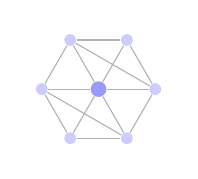
\begin{tikzpicture}[scale=0.6, baseline=(current bounding box.center)]
            % Invisible bounding box for consistent height
            \path[use as bounding box] (-1.5,-1.3) rectangle (1.5,1.3);

            \node[circle, fill=blue!40, inner sep=2pt] (c) at (0,0) {};
            % Create nodes
            \foreach \i in {0,60,...,300} {
                \node[circle, fill=blue!20, inner sep=1.5pt] (n\i) at (\i:1.2) {};
            }
            % Connections
            \foreach \i in {0,60,...,300} {
                \draw[gray!60] (c) -- (n\i);
                \pgfmathsetmacro{\nextangle}{int(mod(\i+60,360))}
                \draw[gray!60] (n\i) -- (n\nextangle);
            }
            \draw[gray!60] (n0) -- (n120);
            \draw[gray!60] (n180) -- (n300);
        \end{tikzpicture}

        \vspace{0.1cm}
        \begin{block}{``Small-World'' Structures}
            \footnotesize
            \begin{itemize}
                \item \textbf{Dense Clustering ($C \approx 0.58$):} Concepts are highly interconnected.
                \item \textbf{Recursive:} Frequent backtracking to refine core definitions (e.g., axioms, ethics).
            \end{itemize}
        \end{block}

        % --- RIGHT COLUMN: PRACTICAL (Tree-Like) ---
        \column{0.48\textwidth}
        \centering
        \textbf{\textcolor{green!40!black}{Practical Domains}} \\
        \scriptsize \textit{(Programming Projects, Debugging)}

        \vspace{0.1cm}
        % Mini TikZ: Tree Structure (fixed height container)
        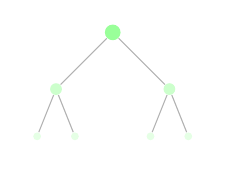
\begin{tikzpicture}[scale=0.6, baseline=(current bounding box.center)]
            % Invisible bounding box for consistent height
            \path[use as bounding box] (-1.8,-1.3) rectangle (1.8,1.3);

            \node[circle, fill=green!40, inner sep=2pt] (root) at (0,1.2) {};
            \node[circle, fill=green!20, inner sep=1.5pt] (l1) at (-1.2, 0) {};
            \node[circle, fill=green!20, inner sep=1.5pt] (r1) at (1.2, 0) {};
            \node[circle, fill=green!10, inner sep=1pt] (l2a) at (-1.6, -1) {};
            \node[circle, fill=green!10, inner sep=1pt] (l2b) at (-0.8, -1) {};
            \node[circle, fill=green!10, inner sep=1pt] (r2a) at (0.8, -1) {};
            \node[circle, fill=green!10, inner sep=1pt] (r2b) at (1.6, -1) {};

            \draw[gray!60] (root) -- (l1);
            \draw[gray!60] (root) -- (r1);
            \draw[gray!60] (l1) -- (l2a);
            \draw[gray!60] (l1) -- (l2b);
            \draw[gray!60] (r1) -- (r2a);
            \draw[gray!60] (r1) -- (r2b);
        \end{tikzpicture}

        \vspace{0.1cm}
        \begin{block}{Tree-Like Expansion}
            \footnotesize
            \begin{itemize}
                \item \textbf{Branching ($C \approx 0.39$):} Task-based exploration without backtracking.
                \item \textbf{Independent:} Projects form isolated silos (e.g., \emph{Metaprogramming} vs. \emph{Physics Sim}).
            \end{itemize}
        \end{block}
    \end{columns}

    \note{
        \textbf{Slide 8: Insight 1 - Heterogeneity (1.5 min)}
        \begin{itemize}
            \item \textbf{Opening - The Big Idea (15s):} ``Here's the first major finding: not all knowledge looks the same. Different domains have fundamentally different \textit{shapes}.''
            \item \textbf{Point to Table - Metrics (20s):} [GESTURE TO TABLE] ``Look at these numbers. Theoretical domains: clustering coefficient 0.58. Practical domains: 0.39. That's a massive difference. Path length also differs---2.3 versus 3.1.''
            \item \textbf{Point to LEFT - Theory Diagram (30s):} [GESTURE TO LEFT DIAGRAM] ``Theoretical topics---math, philosophy, ML theory---are `Small-World' structures. Look at this dense mesh. High clustering. Why? You define a concept, you reuse it across many conversations, you refine it. Recursive thinking. Lots of backtracking and cross-references.''
            \item \textbf{Point to RIGHT - Practice Diagram (30s):} [GESTURE TO RIGHT DIAGRAM] ``Practical coding? Tree-like. Lower clustering. You solve Bug A, move to Bug B. Branching, forward exploration. Projects are isolated---my physics sim doesn't talk to my web dev project. Different cognitive patterns entirely.''
            \item \textbf{Significance (15s):} ``This structural heterogeneity---this within-network diversity---is unique to conversation networks. You don't see this in homogeneous citation networks.''
        \end{itemize}
    }
\end{frame}

%---------------------------------------------------------
% 9. Insight 2: A Taxonomy of Bridges
%---------------------------------------------------------
\begin{frame}{Insight 2: A Taxonomy of Bridges}
    \begin{columns}[T]
        \column{0.55\textwidth}
        \centering
        \includegraphics[width=\textwidth, height=0.8\textheight, keepaspectratio]{images/bridge-better.png}

        \column{0.45\textwidth}
        \textit{The network reveals three distinct bridging mechanisms.}
        \vspace{0.2cm}

        \textcolor{blue}{\textbf{1. Evolutionary Bridges}} \\
        { \scriptsize
        \textit{(e.g., Geometric Mean)}\\
        Conversations that \textbf{drift} from one topic to another (Math $\rightarrow$ AI).
        }
        \vspace{0.2cm}

        \textcolor{teal}{\textbf{2. Integrative Bridges}} \\
        { \scriptsize
        \textit{(e.g., AI Ethics)}\\
        Deliberate synthesis of two fields.
        }
        \vspace{0.2cm}

        \textcolor{orange!80!black}{\textbf{3. Pure Bridges}} \\
        { \scriptsize
        \textit{(e.g., CUDA Linux)}\\
        \textbf{Cognitive Wormholes.} Rare shortcuts through conceptual space (e.g., Gaming $\leftrightarrow$ Coding).
        }
    \end{columns}

    \note{
        \textbf{Slide 9: Insight 2 - Bridge Taxonomy (1.5 min)}
        \begin{itemize}
            \item \textbf{Opening Question (15s):} ``Second finding: How do ideas move between these isolated knowledge islands? The network reveals three distinct bridging mechanisms.''
            \item \textbf{Point to Visualization (15s):} [GESTURE TO LEFT IMAGE] ``This visualization shows high-betweenness nodes---the bridges. Notice they're not all the same type.''
            \item \textbf{Type 1 - Evolutionary (30s):} ``First: Evolutionary Bridges. Conversations that \textit{drift}. The `Geometric Mean' conversation started in pure mathematics, drifted through probability theory, ended up in neural networks. Natural topic evolution. You didn't plan to cross domains---it just happened through the flow of ideas.''
            \item \textbf{Type 2 - Integrative (30s):} ``Second: Integrative Bridges. Deliberate synthesis. `AI Ethics' explicitly brings together technical machine learning knowledge and philosophical frameworks. You're consciously building connections.''
            \item \textbf{Type 3 - Pure Bridges (20s):} ``Third: Pure Bridges---we call them Cognitive Wormholes. A single conversation connecting otherwise distant clusters. Example: a Linux configuration question linking a gaming project to a work project. Rare, but powerful shortcuts through conceptual space.''
            \item \textbf{Bridge (5s):} ``These bridges---these connections across domains---are precisely what makes the map useful. Here's why...''
        \end{itemize}
    }
\end{frame}

%---------------------------------------------------------
% 10. The Vision: Personal Knowledge Cartography
%---------------------------------------------------------
\begin{frame}{The Vision: Personal Knowledge Cartography}
    \centering
    \textbf{Why do we need this map?}

    \vspace{0.05cm}

    % The Graphic: Reduced scale to 0.7 to fit slide
    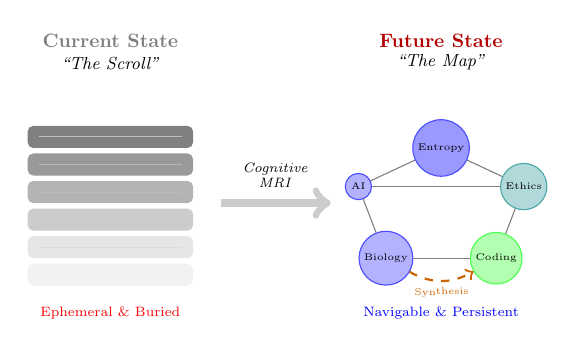
\begin{tikzpicture}[scale=0.7, transform shape]
        % --- LEFT SIDE: THE SCROLL (Current State) ---
        \node[anchor=south] at (1.5, 4.2) {\textbf{\textcolor{gray}{Current State}}};
        \node[anchor=south] at (1.5, 3.8) {\small \textit{``The Scroll''}};

        % Draw a stack of fading bars
        \foreach \y/\opacity in {0/0.1, 0.5/0.2, 1.0/0.4, 1.5/0.6, 2.0/0.8, 2.5/1.0} {
            \draw[fill=gray, opacity=\opacity, draw=none, rounded corners=2pt]
                (0, \y) rectangle (3, \y+0.4);
            \draw[gray!50, opacity=\opacity] (0.2, \y+0.2) -- (2.8, \y+0.2);
        }

        % Label for the problem
        \node[align=center, font=\scriptsize, text=red] at (1.5, -0.5)
            {Ephemeral \& Buried};

        % --- ARROW: THE TRANSFORMATION ---
        \draw[->, line width=1mm, gray!40] (3.5, 1.5) -- (5.5, 1.5);
        \node[font=\scriptsize, align=center] at (4.5, 2) {\textit{Cognitive}\\ \textit{MRI}};

        % --- RIGHT SIDE: THE MAP (Future State) ---
        \node[anchor=south] at (7.5, 4.2) {\textbf{\textcolor{red!70!black}{Future State}}};
        \node[anchor=south] at (7.5, 3.8) {\small \textit{``The Map''}};

        % Define nodes (colors match cluster-vis theoretical/practical palette)
        \node[circle, fill=blue!30, draw=blue!70, inner sep=2pt, font=\tiny] (bio) at (6.5, 0.5) {Biology};
        \node[circle, fill=green!30, draw=green!70, inner sep=2pt, font=\tiny] (code) at (8.5, 0.5) {Coding};
        \node[circle, fill=blue!40, draw=blue!70, inner sep=2pt, font=\tiny] (entropy) at (7.5, 2.5) {Entropy};
        \node[circle, fill=blue!30, draw=blue!70, inner sep=2pt, font=\tiny] (ai) at (6, 1.8) {AI};
        \node[circle, fill=teal!30, draw=teal!70, inner sep=2pt, font=\tiny] (ethics) at (9, 1.8) {Ethics};

        % Draw connections
        \draw[gray] (bio) -- (ai);
        \draw[gray] (ai) -- (entropy);
        \draw[gray] (entropy) -- (ethics);
        \draw[gray] (ethics) -- (code);
        \draw[gray] (bio) -- (code);
        \draw[gray] (ai) -- (ethics);

        % Highlight the "Synthesis" path
        \draw[orange!80!black, thick, dashed, ->] (bio) to[bend right=30]
            node[midway, below, sloped, font=\tiny, text=orange!80!black] {Synthesis} (code);

        % Label for the solution
        \node[align=center, font=\scriptsize, text=blue] at (7.5, -0.5)
            {Navigable \& Persistent};
    \end{tikzpicture}

    \vspace{0.1cm}

    % Concrete example box
    \begin{tcolorbox}[colback=blue!5, colframe=blue!40, boxrule=0.5pt, arc=2pt, left=3pt, right=3pt, top=2pt, bottom=2pt]
        \scriptsize
        \textbf{Example Query:} \textit{``Show me everywhere I discussed entropy.''} \\
        \textbf{Result:} Network lights up connections: Biology $\leftrightarrow$ AI Theory $\leftrightarrow$ Coding $\leftrightarrow$ Ethics
    \end{tcolorbox}

    \vspace{0.05cm}

    % Simplified text - just the core contrast
    \begin{columns}[T]
        \column{0.5\textwidth}
        \centering
        \scriptsize
        \textbf{Problem:} Insights buried \\in infinite scroll

        \column{0.5\textwidth}
        \centering
        \scriptsize
        \textbf{Solution:} Navigate \& synthesize \\across your entire history
    \end{columns}

    \note{
        \textbf{Slide 10: Vision - Personal Knowledge Cartography (50s)}
        \begin{itemize}
            \item \textbf{Opening Question (10s):} ``Why do we need this map?''
            \item \textbf{Point to LEFT - The Problem (20s):} [GESTURE TO SCROLL GRAPHIC] ``Right now, this is how we interact with our AI conversations. An infinite scroll. Linear. Ephemeral. That brilliant insight you had three months ago? Buried somewhere in the timeline. Lost.''
            \item \textbf{Point to ARROW - Transformation (5s):} [GESTURE TO ARROW] ``The Cognitive MRI transforms this...''
            \item \textbf{Point to RIGHT - The Vision (15s):} [GESTURE TO MAP] ``...into this. A navigable map of your knowledge. Imagine asking: `Show me everywhere I discussed entropy.' The network lights up. You see how entropy connected to biology, to your coding projects, to AI ethics discussions. All the cross-connections you forgot about.''
        \end{itemize}
    }
\end{frame}

%---------------------------------------------------------
% 11. Conclusion & Impact
%---------------------------------------------------------
\begin{frame}[fragile]{Cognitive MRI: A Proof of Concept}
    \begin{columns}[T]
        % COLUMN 1: FINDINGS
        \column{0.31\textwidth}
        \begin{exampleblock}{Key Findings}
            \centering
            \includegraphics[width=0.5\textwidth]{images/cluster-vis-topics-better.png}
            \vspace{0.02cm}
            \begin{itemize}
                \scriptsize
                \item \textbf{Method:} User-weighted embedding + Adaptive Thresholding.
                \item \textbf{Topology:} Heterogeneous (Hubs vs. Trees).
                \item \textbf{Bridges:} Evolutionary, Integrative, \& Pure.
            \end{itemize}
        \end{exampleblock}

        \hspace{0.01\textwidth}

        % COLUMN 2: LIMITATIONS
        \column{0.31\textwidth}
        \begin{alertblock}{Limitations}
            \centering
            \vspace{0.02cm}
            % TikZ: Single user with snapshot camera
            \begin{tikzpicture}[scale=0.9]
                % Main user circle with N=1 inside
                \node[circle, fill=red!30, draw=red!60, thick, inner sep=16pt] (user) at (0,0) {};
                \node[font=\Large] at (0,0.15) {\faUser};
                \node[font=\scriptsize, text=red!80] at (0,-0.5) {N=1};
                % Camera icon for "snapshot"
                \node[font=\small, text=gray] at (1.5,1.0) {\faCamera};
            \end{tikzpicture}
            \vspace{0.02cm}
            \begin{itemize}
                \scriptsize
                \item Single User \& Platform.
                \item Snapshot in time.
                \item Exploratory (No ``Ground Truth'').
            \end{itemize}
        \end{alertblock}

        \hspace{0.01\textwidth}

        % COLUMN 3: FUTURE
        \column{0.31\textwidth}
        \begin{block}{Future Directions}
            \centering
            \vspace{0.02cm}
            % TikZ: Growth from 1 to many with temporal evolution + validation
            \begin{tikzpicture}[scale=0.85]
                % Single node on left
                \node[circle, fill=blue!30, draw=blue!60, thick, inner sep=3pt] (one) at (0,0) {};
                % Big arrow with "time" label
                \draw[->, very thick, gray!50] (0.4,0) -- (2.2,0);
                \node[font=\tiny, text=gray, above] at (1.3,0.1) {scale + time};
                % Multiple nodes on right - varying sizes for diversity
                \node[circle, fill=green!40, draw=green!70, thick, inner sep=4pt] at (2.8, 0.7) {};
                \node[circle, fill=green!30, draw=green!60, thick, inner sep=3pt] at (3.2, 0) {};
                \node[circle, fill=green!40, draw=green!70, thick, inner sep=3.5pt] at (2.8, -0.7) {};
                \node[circle, fill=green!20, draw=green!50, thick, inner sep=2.5pt] at (3.7, 0.4) {};
                \node[circle, fill=green!35, draw=green!65, thick, inner sep=3pt] at (3.7, -0.4) {};
                % Connection lines showing network
                \draw[gray!40] (2.8,0.7) -- (3.2,0) -- (2.8,-0.7);
                \draw[gray!40] (3.2,0) -- (3.7,0.4);
                \draw[gray!40] (3.2,0) -- (3.7,-0.4);
                % Validation: magnifying glass examining the network
                \node[font=\normalsize, text=blue!60] at (4.3, 0) {\faSearch};
            \end{tikzpicture}
            \vspace{0.02cm}
            \begin{itemize}
                \scriptsize
                \item \textbf{Scale:} Multi-user cohorts \& cross-platform analysis.
                \item \textbf{Longitudinal:} Track knowledge evolution over time.
                \item \textbf{Validation:} Permutation tests, retrieval benchmarks, user studies.
            \end{itemize}
        \end{block}
    \end{columns}

    \vspace{0cm}
    \centering
    \tiny \faGithub\ \texttt{github.com/queelius/chatgpt-complex-net}
\end{frame}

% NOTE: Placed OUTSIDE frame because [fragile] frames cannot contain \note
\note{
    \textbf{Slide 11: Conclusion - Proof of Concept (1 min)}
    \begin{itemize}
        \item \textbf{Opening Summary (20s):} ``We've demonstrated a proof of concept: LLM conversation logs can be transformed into meaningful cognitive maps showing the latent structure of knowledge.''
        \item \textbf{Point to LEFT - Key Findings (20s):} [GESTURE TO NETWORK IMAGE] ``User-weighted embeddings to capture intent. Heterogeneous topology---theoretical domains look fundamentally different from practical ones. A taxonomy of three bridge types. All validated through rigorous 2D ablation studies.''
        \item \textbf{Point to MIDDLE - Acknowledge Limits (10s):} [GESTURE TO N=1 ICON] ``This is N=1. A single user, single platform, snapshot in time. No ground truth validation yet.''
        \item \textbf{Point to RIGHT - The Path Forward (10s):} [GESTURE TO GROWTH DIAGRAM] ``But those limitations point the way forward. Scale to cohorts. Track longitudinal evolution. Validate with permutation tests and retrieval benchmarks.''
        \item \textbf{Closing (5s):} ``Thank you. Happy to take questions.''
    \end{itemize}
}

%---------------------------------------------------------
% BACKUP SLIDE: Technical Details (for Q&A only)
%---------------------------------------------------------
\begin{frame}[noframenumbering]{Backup: Technical Details}
    \textbf{Embedding Details}
    \begin{itemize}
        \scriptsize
        \item Model: \texttt{nomic-embed-text} (8k context window)
        \item Dimension: 768
        \item Chunking: 500-token windows with 50-token overlap
        \item User-to-AI weighting: 2:1 ratio (validated via ablation study)
    \end{itemize}

    \vspace{0.3cm}

    \textbf{Community Detection}
    \begin{itemize}
        \scriptsize
        \item Algorithm: Louvain (resolution = 1.0)
        \item Modularity: Q = 0.750 (15 communities discovered)
        \item Giant component: 449 nodes, 1,615 edges
    \end{itemize}

    \vspace{0.3cm}

    \textbf{Dataset Filtering}
    \begin{itemize}
        \scriptsize
        \item Original dataset: 1,908 conversations (2 years)
        \item After similarity threshold ($\theta=0.9$): 449 conversations in giant component
        \item Isolated nodes filtered: conversations with no semantic neighbors
    \end{itemize}

    \vspace{0.3cm}

    \centering
    \footnotesize
    \textbf{Full methodology \& code:} \faGithub\ \texttt{github.com/queelius/chatgpt-complex-net}
\end{frame}

%---------------------------------------------------------
% BACKUP SLIDE 2: Core Formulas (for Q&A only)
%---------------------------------------------------------
\begin{frame}[noframenumbering]{Backup: Core Formulas}

    \begin{columns}[T]
        \column{0.5\textwidth}
        \small

        \textbf{Weighted Embedding}
        \vspace{-0.1cm}
        \begin{equation*}
            \footnotesize
            \vec{e}_{conv} = \frac{\alpha \vec{e}_{user} + \vec{e}_{AI}}{\|\alpha \vec{e}_{user} + \vec{e}_{AI}\|}
        \end{equation*}
        \vspace{-0.15cm}
        {\scriptsize $\alpha = 2$ (2:1 weighting)}

        \vspace{0.3cm}

        \textbf{Modularity (Newman's Q)}
        \vspace{-0.1cm}
        \begin{equation*}
            \footnotesize
            Q = \frac{1}{2m} \sum_{ij} \left[ A_{ij} - \frac{k_i k_j}{2m} \right] \delta(c_i, c_j)
        \end{equation*}
        \vspace{-0.15cm}
        {\scriptsize $A_{ij}$: adjacency, $k_i$: degree, $m$: edges}

        \column{0.5\textwidth}
        \small

        \textbf{Betweenness Centrality}
        \vspace{-0.1cm}
        \begin{equation*}
            \footnotesize
            B(v) = \sum_{s \neq v \neq t} \frac{\sigma_{st}(v)}{\sigma_{st}}
        \end{equation*}
        \vspace{-0.15cm}
        {\scriptsize $\sigma_{st}$: shortest paths $s \to t$}

        \vspace{0.3cm}

        \textbf{Clustering Coefficient}
        \vspace{-0.1cm}
        \begin{equation*}
            \footnotesize
            C_i = \frac{2e_i}{k_i(k_i - 1)}
        \end{equation*}
        \vspace{-0.15cm}
        {\scriptsize $e_i$: edges among neighbors}
    \end{columns}

\end{frame}

%---------------------------------------------------------
% BACKUP SLIDE 3: Privacy & Data Handling (for Q&A only)
%---------------------------------------------------------
\begin{frame}[noframenumbering]{Backup: Privacy \& Data Handling}
    \begin{columns}[T]
        \column{0.5\textwidth}
        \textbf{This Study}
        \begin{itemize}
            \scriptsize
            \item \textbf{Consent:} Author's own conversations
            \item \textbf{Export:} Official ChatGPT data export
            \item \textbf{Content:} Exploratory/academic only
            \item \textbf{Sharing:} Aggregated statistics, no raw logs
        \end{itemize}

        \vspace{0.2cm}

        \textbf{Code Release}
        \begin{itemize}
            \scriptsize
            \item Framework is open-source
            \item Users run locally on their own data
            \item No data leaves user's machine
        \end{itemize}

        \column{0.5\textwidth}
        \textbf{Future Multi-User Studies}
        \begin{itemize}
            \scriptsize
            \item \textbf{IRB Required:} Formal ethics review
            \item \textbf{Informed Consent:} Explicit opt-in
            \item \textbf{Anonymization:}
                \begin{itemize}
                    \tiny
                    \item Remove PII (names, emails)
                    \item Hash conversation IDs
                    \item Redact sensitive topics
                \end{itemize}
            \item \textbf{Differential Privacy:} For aggregate statistics
        \end{itemize}

        \vspace{0.2cm}

        \begin{alertblock}{\scriptsize Key Principle}
            \tiny
            Designed for \textbf{self-knowledge}---users mapping their own thought, not surveillance.
        \end{alertblock}
    \end{columns}
\end{frame}

%---------------------------------------------------------
% BACKUP SLIDE 4: Methodology Alternatives (for Q&A only)
%---------------------------------------------------------
\begin{frame}[noframenumbering]{Backup: Methodology Alternatives}
    \textbf{Why These Design Choices?}

    \vspace{0.1cm}

    \scriptsize
    \begin{tabular}{@{}p{2.2cm}p{2.5cm}p{5cm}@{}}
        \toprule
        \textbf{Choice} & \textbf{Alternative} & \textbf{Why We Chose This} \\
        \midrule
        \textbf{Cosine Similarity} & Euclidean Distance & Magnitude-invariant (length $\neq$ relevance) \\
        & Jaccard (set-based) & Semantic continuity, not just keywords \\
        \midrule
        \textbf{Threshold} ($\theta$=0.9) & Soft/fuzzy clustering & Clear community boundaries \\
        & k-NN graph & Ablation validated hard threshold \\
        \midrule
        \textbf{nomic-embed-text} & OpenAI embeddings & Open weights, 8k context, reproducible \\
        & Sentence-BERT & Better long-context handling \\
        \midrule
        \textbf{2:1 Weighting} & Equal (1:1) & AI responses dilute user intent \\
        & User-only & Loses conversational context \\
        \bottomrule
    \end{tabular}

    \vspace{0.2cm}

    \centering
    \tiny
    \textit{All choices validated via 63-configuration ablation study (Slide 6)}
\end{frame}

\end{document}
